\documentclass[../thesis.tex]{subfiles}
\graphicspath{{\subfix{../Images/}}}

\begin{document}

\section{Power Usage experiment results}\label{section:power}
In this section, I will describe the results of the \textbf{Power Usage experiments}. First, I measured the power consumption while using the pre-trained neural network SqueezeNet \parencite{sqnet}, after this abbreviated to sqnet. I will describe the measurements in \autoref{subsection:sqnet}. The power readings for Cheetah can be found in \autoref{fig:mean_cheetah_sqnet}, and the measurements of $SCI_{HE}$ can be found in \autoref{fig:mean_SCI_HE_sqnet}. Additionally, I measured the power consumption while using the pre-trained neural network ResNet50 \parencite{resnet}, after this described as resnet50. I will describe the measurements in \autoref{subsection:resnet}. The power readings for Cheetah can be found in \autoref{fig:mean_cheetah_resnet50}, and the measurements of $SCI_{HE}$ can be found in \autoref{fig:mean_SCI_HE_resnet50}. 

\subsection{SqueezeNet}\label{subsection:sqnet}
\begin{figure}[th!]
    \begin{subfigure}{.75\linewidth}
            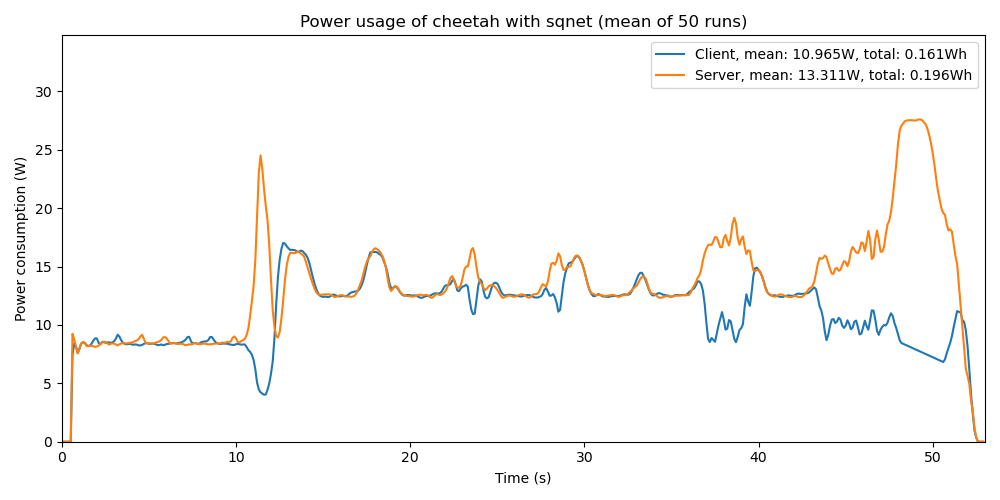
\includegraphics[width=\textwidth]{Thesis/Images/Means/mean_cheetah-sqnet.png}
            \caption{Mean of running Cheetah with sqnet 50 times.}
            \label{fig:mean_cheetah_sqnet}
    \end{subfigure}
    \medskip
    \begin{subfigure}{.75\linewidth}
            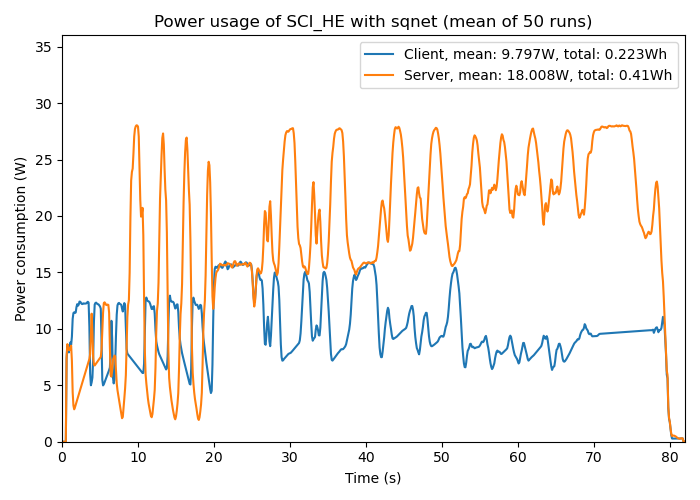
\includegraphics[width=\textwidth]{Thesis/Images/Means/mean_SCI_HE-sqnet.png}
            \caption{Mean of running $SCI_{HE}$ with sqnet 50 times.}
            \label{fig:mean_SCI_HE_sqnet}
    \end{subfigure}

    % \medskip % create some *vertical* separation between the graphs
    % \begin{subfigure}{.475\linewidth}
            % \includegraphics[width=\textwidth]{img}
    % \end{subfigure}
    \caption{Measurements of both SNNI's on NN Sqnet.}
\end{figure}

Cheetah is consuming an average of approximately 8 Watts in approximately the first 10 seconds. There seems to be an interplay between the client and the server in this period, where the average usage is relatively low compared to the period after approximately 10 seconds. $SCI_{HE}$ also shows a phase at the start, in approximately the first 20 seconds, where the average consumption is lower. The server sometimes reaches a power consumption of almost zero in this period, while after 20 seconds the lowest power consumption is at least 10 Watts. 

In the period past 10 seconds, Cheetah shows some peaks and troughs. Some of these peaks for the client align with peaks for the server process. At other places, there are peaks on the server side and troughs on the client side. There seem to be no places with troughs for the server and peaks for the client. $SCI_{HE}$, on the other hand, does have these places. It is harder to see, because the average power consumption of the client is lower compared to the client. However, after 20 seconds, there seem to be no places with peaks for both server and client ant the same time. When the server consumes above average, the client consumes below average, and the other way around. Additionally, $SCI_{HE}$ only has peaks and troughs, while Cheetah seems to have a more constant consumption with some peaks and troughs. 

If one looks at the average power consumption and total energy consumption, there are a few things to point out. First, although the client with Cheetah has a higher power consumption, the energy consumption is lower than the client with $SCI_{HE}$. This could be explained because the relative speed-up is higher than the relative increment of power consumption, and energy is calculated as time multiplied with power. Second, the server protocol consumes almost two times more power and energy compared to the client protocol on $SCI_{HE}$. The client and servers power and energy consumption of Cheetah, on the contrary, are more similar. Third, Cheetah consumes less power compared to $SCI_{HE}$. 

% % One other interesting fact is that the average power consumption of the client and the server is closer for Cheetah than for $SCI_{HE}$. For $SCI_{HE}$, on the other hand, the server almost uses double the amount of power, and also consumes almost double the energy. I do not know what causes this difference, but I think that this could be explained when it is researched what layers cause the peaks and troughs. 
% second,  total power consumption and energy consumption is lowwer for cheetah. While client power consumption is a bit higher, the server is a lot lower. This together with the speedup results in a lower energy consumption
% % Although the client uses more power in Cheetah compared to $SCI_{HE}$, the image shows that the average energy consumption is lower. The reason for this is that Cheetah has a lower run time compared to $SCI_{HE}$. The server uses less power compared to $SCI_{HE}$, and combined with the fact that Cheetah is faster, also has a lower average energy consumption. The difference between the energy consumption is highest for the server, since it consumes less power and has a lower run time, while the client only has a lower run time. 

 
% Remarks on Cheetah:
% \begin{itemize}
%         \item Results Cheetah look very asynchronized, i.e. peaks in power usage on client often mean power troughs. We can see this very good when Cheetah uses the silent OT pack and is synchronising (first 0-10 seconds before the actual inference phase). We can see this best in figure \ref{fig:mean_cheetah_sqnet}. This means that when the server is calculating, the client is running idle.
%         \item There are also places in Cheetah where they run syncrhonous. On these places there are peaks for both client and server power usage, e.g. in figure \ref{fig:mean_cheetah_sqnet} between 15-20 seconds. This means that both client and server are calculating.
%         \item Idle power consumption with cheetah in the synchronising phase of the silent OT pack is around 9 Watts
%         \item Idle power consumption with cheetah in the inference phase is around 12 Watts
%         \item With Cheetah the power consumption of server often has peaks when the client has troughs. This is probably because the server is calculating more things than client. This would explain the higher mean of the server side. 
% \end{itemize}
% Remarks on $SCI_{HE}$:
% \begin{itemize}
%         \item Results $SCI_{HE}$ also look synchronized. See figure \ref{fig:mean_SCI_HE_sqnet}. This means that either the server or the client is calculating.
%         \item I cannot find places where both client and server are calculating. 
%         \item While the mean power consumption of the client on $SCI_{HE}$ is lower then Cheetah, the energy consumption is higher on $SCI_{HE}$ then Cheetah. This is because the average runtime is higher with $SCI_{HE}$.
% \end{itemize}

\subsection{ResNet50}\label{subsection:resnet}
\begin{figure}[th!]
    \begin{subfigure}{.8\linewidth}
            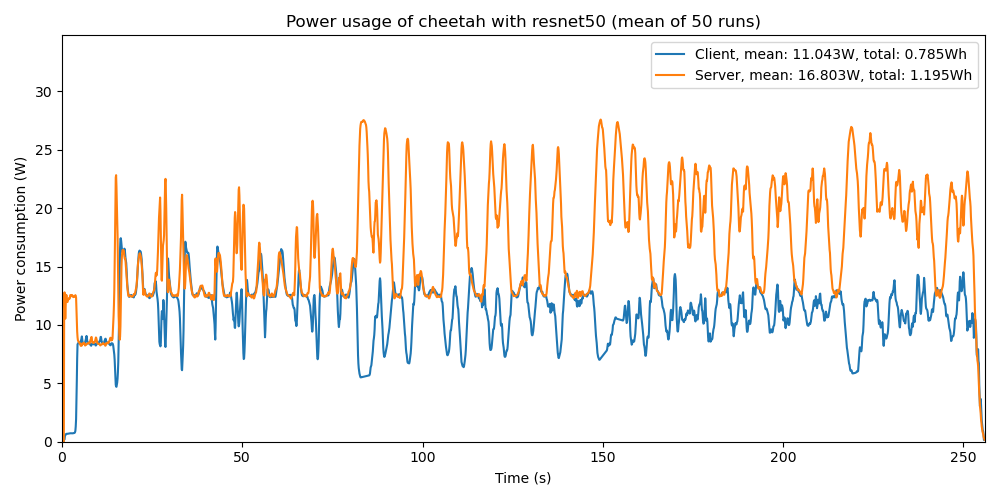
\includegraphics[width=\textwidth]{Thesis/Images/Means/mean_cheetah-resnet50.png}
            \caption{Mean of running Cheetah with resnet50 50 times.}
            \label{fig:mean_cheetah_resnet50}
    \end{subfigure}
    \medskip
    \begin{subfigure}{.8\linewidth}
            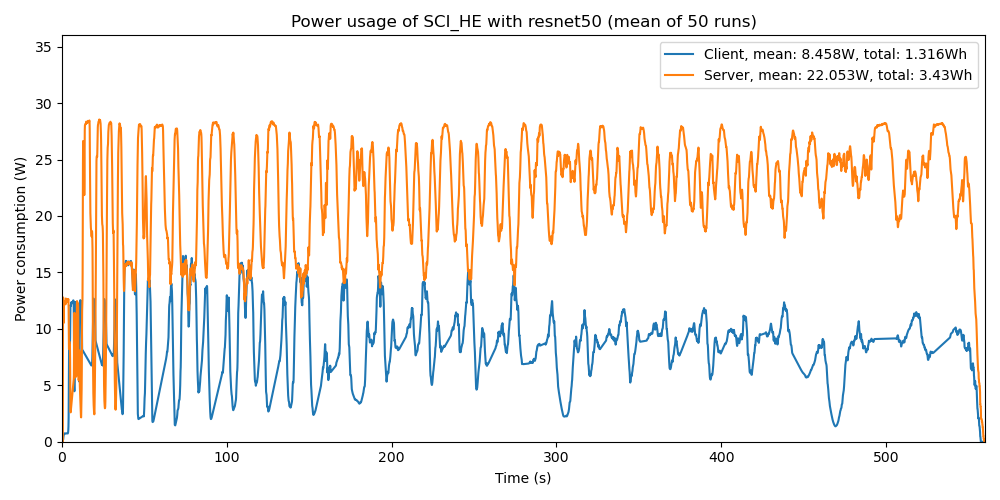
\includegraphics[width=\textwidth]{Thesis/Images/Means/mean_SCI_HE-resnet50.png}
            \caption{Mean of running $SCI_{HE}$ with resnet50 50 times.}
            \label{fig:mean_SCI_HE_resnet50}
    \end{subfigure}

    % \medskip % create some *vertical* separation between the graphs
    % \begin{subfigure}{.475\linewidth}
            % \includegraphics[width=\textwidth]{img}
    % \end{subfigure}
    \caption{Measurements of both SNNI's on NN ResNet50.}
\end{figure}
Although resnet50 is an entirely different NN compared to sqnet (other layers, different amount of layers, e.g. 18 and 50 for sqnet and resnet50 respectively, etc.), the graphs show multiple resemblances. 

% \begin{wrapfigure}{l}{.7\textwidth}
%     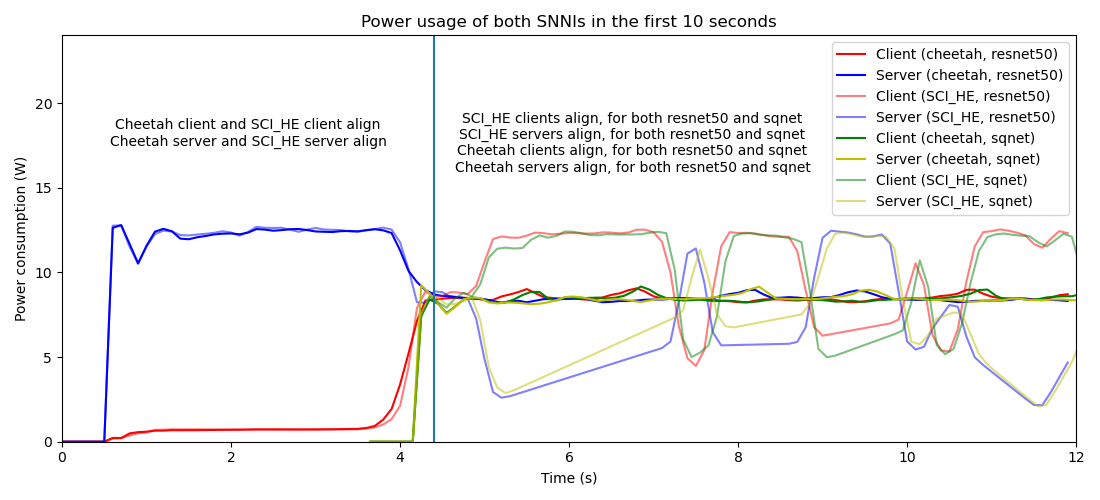
\includegraphics[width=\linewidth]{Thesis/Images/mean_first10secs.png} 
%     \caption{First 10 seconds of both SNNIs and both NNs. Sqnet graph is shifted 3.6 seconds (duration of the Eigen phase).}
%     \label{fig:first10secs}
% \end{wrapfigure}


An example of such resemblance is the phase in approximately the first 10 seconds of Cheetah. Although there seems a high power consumption in the first 4 seconds, the 10 seconds after show an interplay between client and server with an average of 8 Watts again. The same phenomenon as $SCI_{HE}$ with sqnet can be seen with resnet50 in approximately the first 20 seconds. For both SNNIs, there seems to be an offline phase, a phase that is independent of the NN. 

Another example of resemblance is the alignment of peaks. Some of the peaks for Cheetahs client align with peaks for the server process. At other places, there are peaks on the server side and troughs on the client side. Again, no places can be found with troughs for the server and peaks for the client. $SCI_{HE}$, on the other hand, has these places, just like with sqnet. After 20 seconds, there seem to be no places with peaks for both server and client ant the same time. When the server consumes above average, the client seems to consume below average, and the other way around. In addition, Cheetah with resnet50 also seems to have a constant consumption with peaks and troughs, while $SCI_{HE}$ only seems to have peaks and troughs, just like with sqnet. Lastly, the ratio between the power consumption of the server and client is approximately the same; the client and server with Cheetah have almost similar power consumption, while the power consumption of the server is almost double the consumption of the client with $SCI_{HE}$. Additionally, Cheetahs client is more energy efficient compared to $SCI_{HE}$s client, similar for Cheetahs server and $SCI_{HE}$s server.
% \color{red}Offline phase is visible, independent of the NN\color{black}
% The synchronising phase is still visible in Cheetah (see first 10 seconds), and also in $SCI_{HE}$ (see first 20 seconds). One difference is that for Cheetah in the first few seconds (before the synchronising phase), one can see an increase in power usage for the server and a decrease in power usage for the client. $SCI_{HE}$ also shows this, but this is less visible. 








\section{Bandwidth experiment results}

\begin{figure}[hbt]
% \renewcommand{\figurename}{Fig.}
    \begin{floatrow}
        \ffigbox[0.5\textwidth]{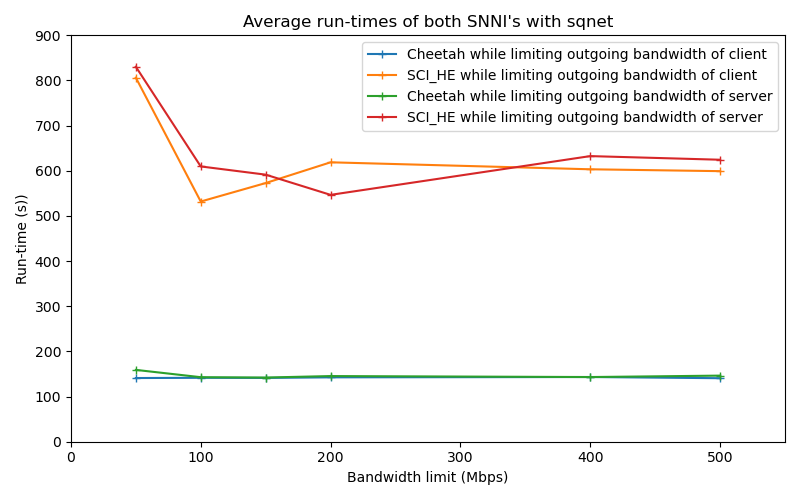
\includegraphics[width=\linewidth]{{Thesis/Images/graph_times_mean.png}}}{
            \caption{Average run-time for both Cheetah and $SCI_{HE}$.}
            \label{fig:graph_times_mean}
        }
        \ffigbox[0.5\textwidth]{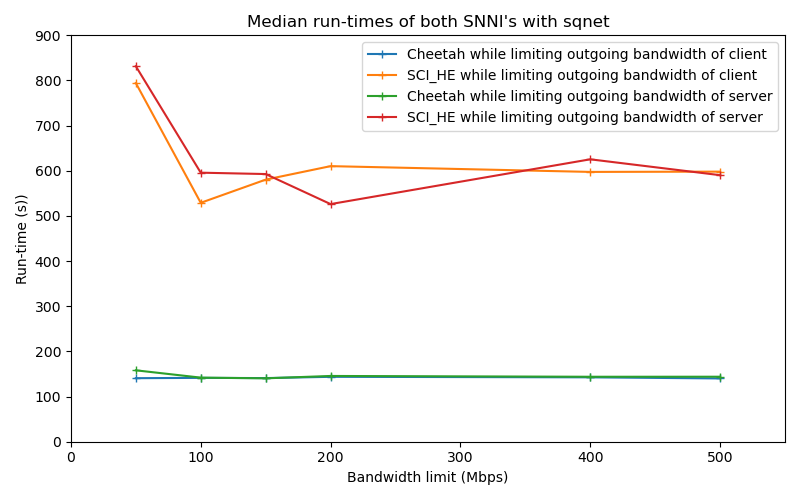
\includegraphics[width=\linewidth]{{Thesis/Images/graph_times_avg.png}}}{
            \caption{Median run-time for both Cheetah and $SCI_{HE}$.}
            \label{fig:graph_times_median}
        }
    \end{floatrow}
\end{figure}
I measured the bandwidth of both SNNI's using the NN sqnet. I performed some experiments using resnet50, but I quickly found that running resnet50 would take a long time\footnote{The lowest run-time of running $SCI_{HE}$ with resnet50 6 times was 9 hours and 9 minutes. The longest run was 14 hours and 42 minutes. The longest run with Cheetah was a little bit under 14 minutes however.}. The results from limiting the bandwidth of the client can be found in \autoref{table:powerreadingsclient}, and the results from limiting the bandwidth of the server can be found in \autoref{table:powerreadingsserver}. For each bandwidth, I ran the SNNI at least 10 times\footnote{With the experiments for limiting the bandwidth of the server, I ran the test 15 times for each bandwidth. These tests took almost a day (23 hours and 45 minutes) to finish. I then down-scaled the experiment and ran the experiment 10 times per bandwidth. This took 13 hours and 45 minutes.} and calculated the mean of these runs. 

These results did not show a significant increase or decrease in energy consumption, which was unexpected. My expectation was that, although the SNNI would not use the maximum bandwidth available, the SNNI would have periods with a high rate of data exchange. I therefore assumed that the limits would have impact on the energy consumption. As can be seen in the tables, the effect is close to zero. One small change that I did find, was in \autoref{table:powerreadingsserver}. It is visible that the overall energy consumption is normally around $0.390$ Wh and $0.950$ Wh for Cheetah and $SCI_{HE}$ respectively. However, in the case of 50 Mbps of available bandwidth, the energy consumption increases somewhat. This could be a case of outliers, however, it could also mean that the energy consumption increases when lowering the available bandwidth under 50 Mbps. 

One other remark can be seen in the run-times of the SNNIs (see \autoref{fig:graph_times_mean}). One can see that the run-time for Cheetah almost stays the same. One small increase can be seen at 50 Mbps, but no other curious characteristics. $SCI_{HE}$, on the other hand, does have curious characteristics. When limiting the client, the run-time increases. This can be explained since limiting bandwidth will increase communication time. When lowering the limit of the bandwidth to 200 Mbps however, the run-time decreases, for it to increase a lot after 100 Mbps. The same phenomenon happens when limiting the server. The run-time decreases when limiting the run-time to 400 Mbps and lowering, but it increases with a limit of 200 Mbps. This could be explained by extreme outliers. But when I graph the medians, so the graph is not skewed by a small proportion of outliers, and almost the same graph can be seen (see \autoref{fig:graph_times_median}). I checked the times on which the tests ran and this gave some insight. The fast run-times (100 and 150 Mbps) when limiting the client's bandwidth were at night-time when no other traffic passed the router. The higher run-times (200 Mbps for example) were in the evening or at day-time, so there could be other traffic passing the router. Same counts for the bandwidth measured at 200 Mbps when limiting the bandwidth of the server, when the experiments were in the evening. Although traffic was minimal\footnote{I unfortunately did not have the means to use the router exclusively for the experiments, so other traffic (although minimal) could have passed the router}, it could have influenced the run-time. Because it is not sure if this influences the run-time, one could perform extra experiments with a router exclusively used for this experiment to see if this is indeed the case. I have not done these experiments because of the limited means available.

\begingroup
    \setlength{\intextsep}{0pt}
    \begin{wraptable}{r}{.25\textwidth}
        \begin{tabular}{ll}
                Generation & Bandwidth \\ \hline
                5G         & 100Mbits  \\ \hline
                LTE        & 30Mbits   \\ \hline
                4G         & 14Mbits   \\ \hline
                3G         & 3Mbits   
        \end{tabular}
        \caption{Average bandwidth of Cellular Broadband Connections.}
        \label{table:bandwidth}
    \end{wraptable}

The run-time with a limit of 50 Mbps can not be explained by the time of the experiment however, since the conditions were optimal (tests done at night-time). According to \autoref{table:powerreadingsclient} and \autoref{table:powerreadingsserver}, it is shown that the energy consumption does also increase when limiting the bandwidth to 50 Mbps for $SCI_{HE}$, compared to the other limits for $SCI_{HE}$. I did check the average data exchanged for both SNNIs, without limiting the bandwidth of either the server or the client. The data exchanged for Cheetah was between 11 and 12 Mbps, and the average data exchanged for $SCI_{HE}$ was between 40 and 60 Mbps. This explains why limiting the bandwidth to 100 Mbps or higher does have little impact on the average run-time and energy consumption. I thought that, although the average is around 50 Mbps, the SNNI is sometimes in a computing phase (with no communication) and sometimes in a communication phase (which increases the average), and that lowering the amount of available bandwidth till 50 Mbps would also impact the energy consumption.  

Since limits higher than 100 Mbps seem to have little to no impact on the energy consumption, I decided to perform extra experiments. The bandwidth limits chosen are based on the maximum bandwidth of the cellular broadband generations (table \ref{table:bandwidth}). Any generation lower than 5G should have impact on the energy consumption of $SCI_{HE}$, while any generation lower than LTE should have an impact on Cheetah. I will describe the results in the next section. 
\endgroup
\begin{table}[htb]
    \begin{adjustbox}{width=.9\columnwidth,center}
        \subfile{../Tables/Power_readings_client}
    \end{adjustbox}
    \caption{Power readings of running the Cheetah and $SCI_{HE}$ and limiting the outgoing bandwidth of the client.}
    \label{table:powerreadingsclient}
\end{table}

\begin{table}[htbp]
    \begin{adjustbox}{width=.9\columnwidth,center}
        \subfile{../Tables/Power_readings_server}
    \end{adjustbox}
    \caption{Power readings of running the Cheetah and $SCI_{HE}$ and limiting the outgoing bandwidth of the server.}
    \label{table:powerreadingsserver}
\end{table}



\subsection{Using lower bandwidth limits}\label{subsection:lowerbw}
\begingroup
    \setlength{\intextsep}{0pt}
    \setlength{\columnsep}{0pt}
    \begin{wrapfigure}{r}{.6\textwidth}
        \centering
        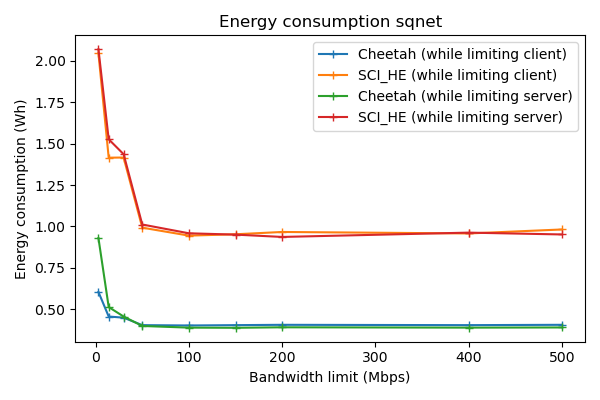
\includegraphics[width=\linewidth]{Thesis/Images/graph_means.png}
        \caption{Average energy consumption.}
        \label{fig:avg_energy}
    \end{wrapfigure}
    
Because of the limited available time, I performed the tests at least 5 times\footnote{Limiting bandwidth of the server tests done 10 times, and limiting the bandwidth of the client 5 times}. Results can be found in \autoref{table:powerreadingsclient2} and \autoref{table:powerreadingsserver2}. The results of this experiment, together with the limits higher than 50 Mbps, can also be found in \autoref{fig:avg_energy}.

As can be seen in \autoref{fig:avg_energy}, the energy consumption indeed increases when the bandwidth limit is lower than 50 Mbps and 100 Mbps for Cheetah and $SCI_{HE}$ respectively. The graph for limiting the server does look smooth, while the graph for limiting the client shows a bump at 14 Mbps, both for Cheetah and $SCI_{HE}$. 

In both \autoref{fig:avg_energy} and \autoref{table:powerreadingsclient2} it is shown that the improvement of energy consumption for cheetah compared to the energy consumption of $SCI_{HE}$ increased when lowering the available bandwidth of the client. In the \autoref{fig:avg_energy} and \autoref{table:powerreadingsclient2} it is shown that the improvement is better when limiting the available bandwidth of the client compared to limiting the bandwidth of the server. The improvement of the client decreases when limiting the client's bandwidth. The improvement of the server, on the other hand, increases. When limiting the servers outgoing bandwidth, there is no increment or decrement visible for both the server and the client. 

 
\endgroup
\begingroup
    \setlength{\intextsep}{10pt}
    \setlength{\columnsep}{0pt}
\begin{table}[ht]
        \begin{adjustbox}{width=\columnwidth,center}
                \subfile{../Tables/Power_readings_client2}
        \end{adjustbox}
        \caption{Power readings of running the Cheetah and $SCI_{HE}$ and limiting the outgoing bandwidth of the client.}
        \label{table:powerreadingsclient2}
\end{table}

\begin{table}[ht]
        \begin{adjustbox}{width=\columnwidth,center}
                \subfile{../Tables/Power_readings_server2}
        \end{adjustbox}
        \caption{Power readings of running the Cheetah and $SCI_{HE}$ and limiting the outgoing bandwidth of the server.}
        \label{table:powerreadingsserver2}
\end{table}
\endgroup

% \newpage
% \subsection{Lowering bandwidth of both devices}

% \begin{table}[ht]
%         \begin{adjustbox}{width=\columnwidth,center}
%                 \subfile{../Tables/Power_readings_both}
%         \end{adjustbox}
%         \caption{Power readings of running the Cheetah and $SCI_{HE}$ and limiting the outgoing bandwidth of both client and server at the same time.}
%         \label{table:powerreadingsboth}
% \end{table}
% Remarks:
% \begin{itemize}
%     \item Increase of speedup for cheetah. Lower energy consumption. 
%     \item Increase can be seen mainly on server side, on client side it decreases
%     \item Highest energy consumption on server side on 3Mbits
% \end{itemize}

% \section{RQb, how does the bandwidth influence the energy consumption of a SNNI}

% \subsection{graphs}
% \begin{figure}[hbt!]
%     \begin{subfigure}{.475\linewidth}
%             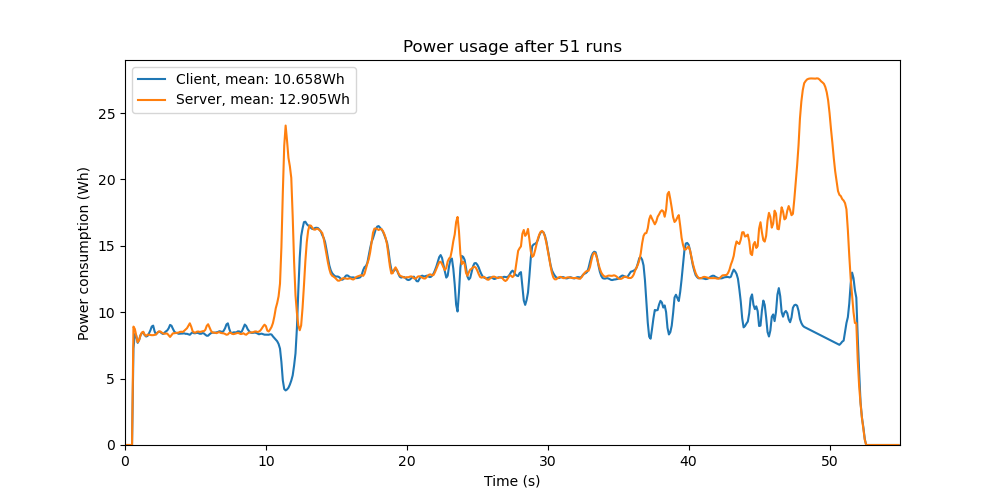
\includegraphics[width=\textwidth]{Thesis/Images/Means/mean_cheetah_resnet50.png}
%             \caption{Mean of running Cheetah with resnet50 51 times}
%             \label{fig:mean_cheetah_resnet50}
%     \end{subfigure}\hfill % <-- "\hfill"
%     \begin{subfigure}{.475\linewidth}
%             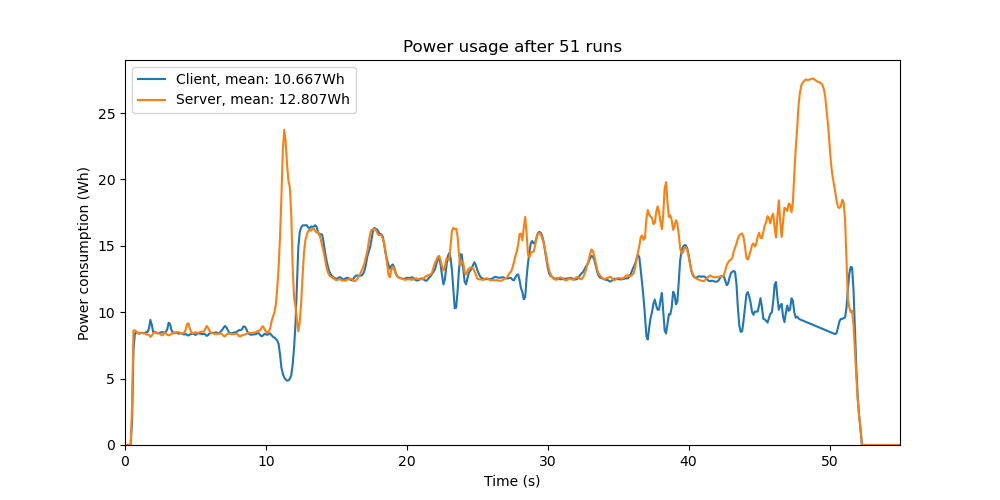
\includegraphics[width=\textwidth]{Thesis/Images/Means/mean_cheetah_sqnet.png}
%             \caption{Mean of running Cheetah with sqnet 51 times}
%             \label{fig:mean_cheetah_sqnet}
%     \end{subfigure}

%     \medskip % create some *vertical* separation between the graphs
    
%     \begin{subfigure}{.475\linewidth}
%             \includegraphics[width=\textwidth]{Thesis/Images/Means/mean_SCI_{HE}_sqnet.png}
%             \caption{Mean of running SCI\_HE with sqnet 11 times}
%             \label{fig:mean_SCI_{HE}_sqnet}
%     \end{subfigure}\hfill % <-- "\hfill"
%     \begin{subfigure}{.475\linewidth}
%             \includegraphics[width=\textwidth]{Thesis/Images/Means/mean_SCI_{HE}_sqnet.png}
%             \caption{Mean of running SCI\_HE with sqnet 11 times}
%             \label{fig:fmean_SCI_{HE}_sqnet}
%     \end{subfigure}

%     \caption{Four measurements doneA figure with four subfigures}
%     \label{fig:4results}
% \end{figure}

% \begin{figure}[hbt!]
%     \begin{subfigure}{\linewidth}
%             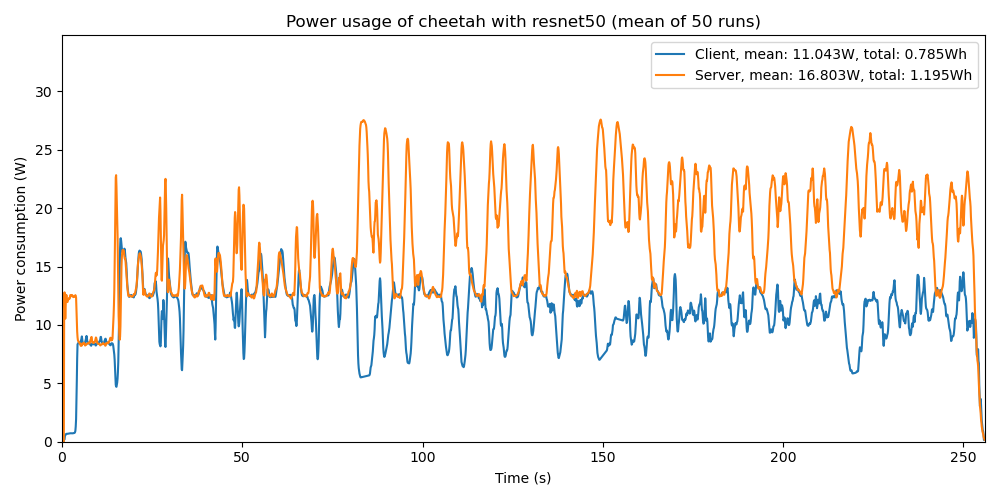
\includegraphics[width=\textwidth]{Thesis/Images/Means/mean_cheetah-resnet50.png}
%             \caption{Mean of running Cheetah with resnet50 51 times}
%             \label{fig:bmean_cheetah_resnet50}
%     \end{subfigure}
%     \begin{subfigure}{\linewidth}
%             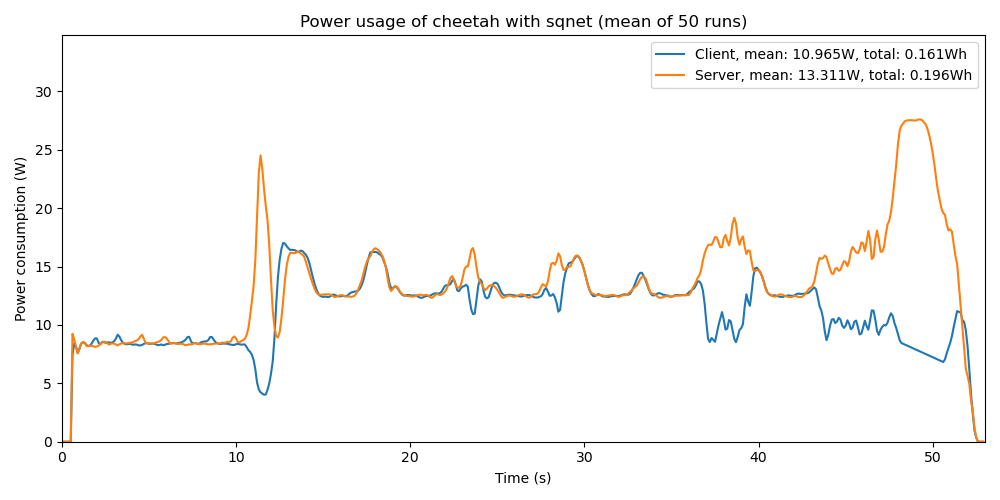
\includegraphics[width=\textwidth]{Thesis/Images/Means/mean_cheetah-sqnet.png}
%             \caption{Mean of running Cheetah with sqnet 51 times}
%             \label{fig:bmean_cheetah_sqnet}
%     \end{subfigure}    
%     \begin{subfigure}{\linewidth}
%             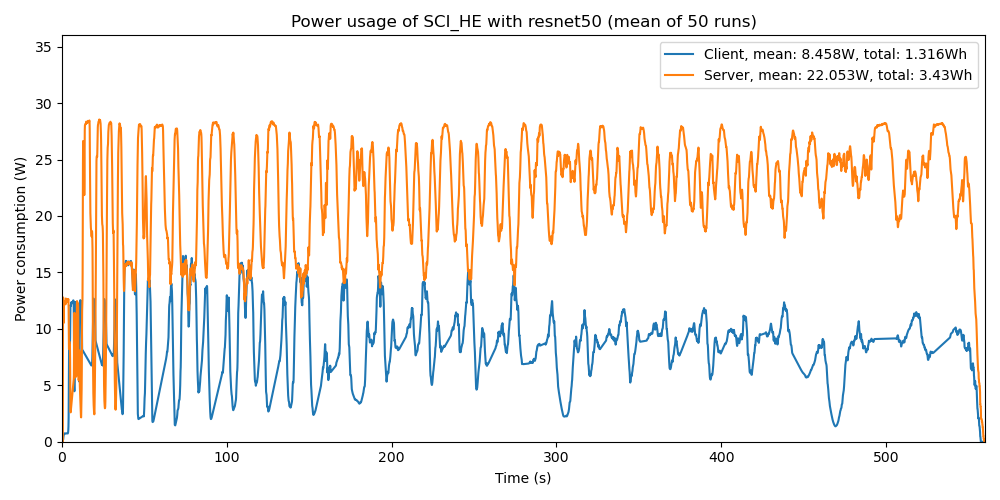
\includegraphics[width=\textwidth]{Thesis/Images/Means/mean_SCI_HE-resnet50.png}
%             \caption{Mean of running SCI\_HE with sqnet 11 times}
%             \label{fig:bmean_SCI_{HE}_sqnet}
%     \end{subfigure}
%     \begin{subfigure}{\linewidth}
%             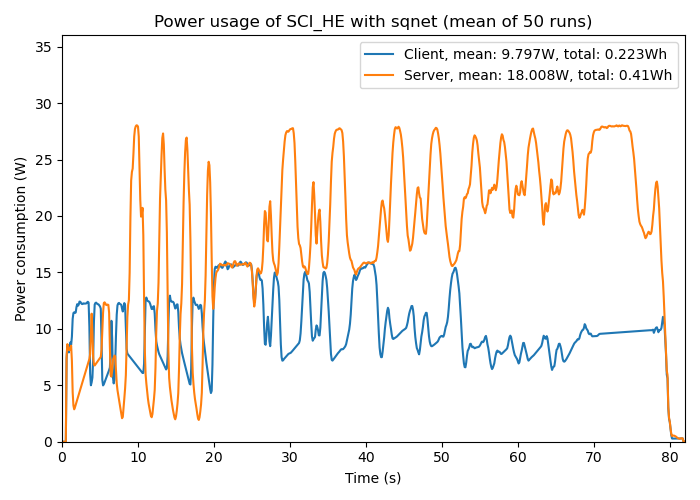
\includegraphics[width=\textwidth]{Thesis/Images/Means/mean_SCI_HE-sqnet.png}
%             \caption{Mean of running SCI\_HE with sqnet 11 times}
%             \label{fig:bfmean_SCI_{HE}_sqnet}
%     \end{subfigure}

%     \caption{Four measurements doneA figure with four subfigures}
%     \label{fig:4results2}
% \end{figure}

% \noindent
% Cross-references to subfigures \ref{fig:mean_cheetah_resnet50}, \ref{fig:mean_cheetah_sqnet} and \ref{fig:mean_SCI_{HE}_sqnet} and of figure \ref{fig:4results}.

% \begin{figure}[h!]
%     \centering
%     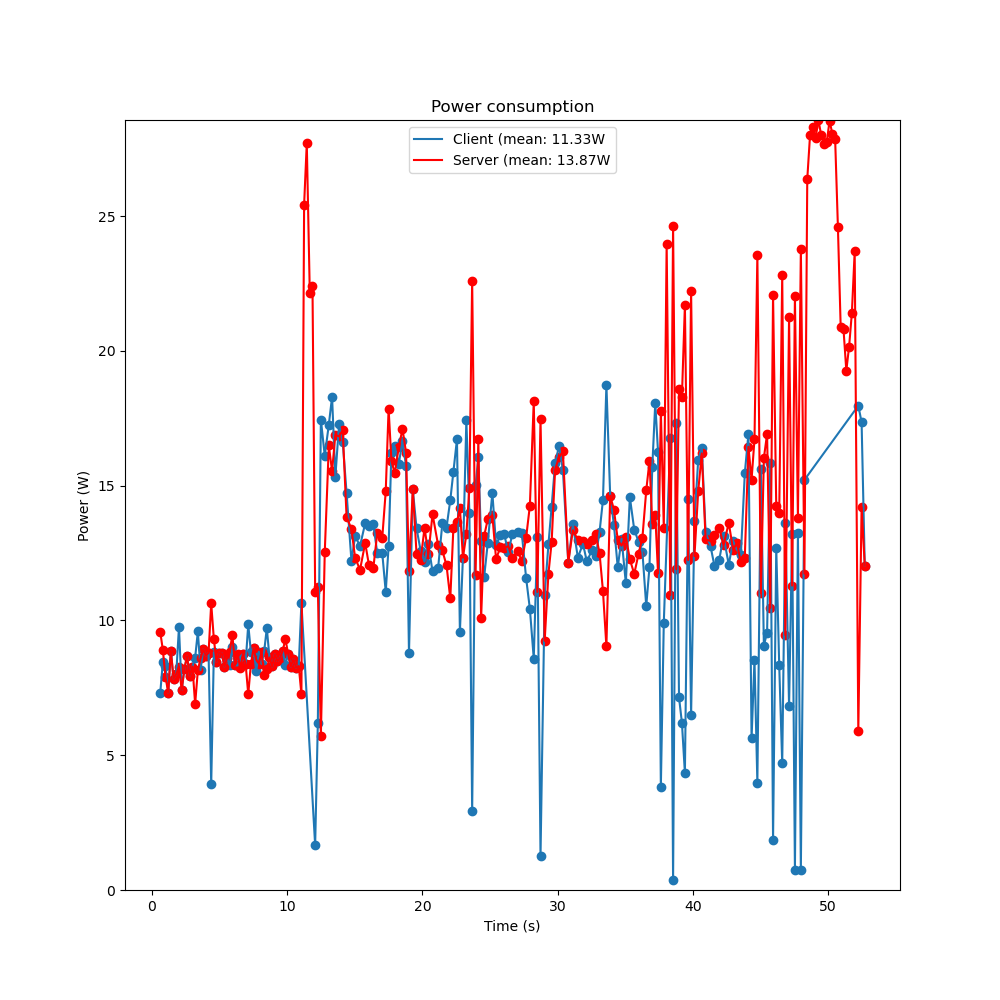
\includegraphics[width=\textwidth,height=\textheight,keepaspectratio]{cheetah-sqnet.png}
%     \caption{Running the SNNI cheetah on sqnet}
%     \label{fig:my_label}
% \end{figure}
% \newpage
% \begin{figure}[h!]
%     \centering
%     \includegraphics[width=\textwidth,height=\textheight,keepaspectratio]{SCI_{HE}-sqnet.png}
%     \caption{Running the SNNI CrypTFlow2 on sqnet}
%     \label{fig:my_label}
% \end{figure}
% \section{RQb, what are the differences on server and client side and what are the implications}
\end{document}
